\subsection{Cykelbane som løsningforslag for et tryggere område i Nytorv}
\label{sub:Cykelbane_som_loesningforslag_for_et_tryggere_omraade_i_Nytorv}
I dette afsnit er forskellen på en cykelsti og cykelbane beskrevet, da de har hver deres udformning, men kan oftest opfattes ens.  Dermed er der foretaget nogle mål og tegninger for, hvordan en ruteplanlægningen kunne se ud i Nytorv/Østerågade og gennem Boulevarden. 

\subsection{Forskellen på cykelsti og cykelbane}
\label{forskelpaacykelstii}
Antallet af cyklister er flere steder vokset meget højt, og nogle steder kan der opleves en vis form for utryghed (se bilag). Ifølge flere interviewpersoner, som medvirkede i interviewet på Nytorv/Østerågade bliver fodgængere og forbigående cyklister utrygge, af manglende plads til cyklisterne på kørebanen i området, hvilket resultere i at cyklisterne benytter sig af fortovet. Derfor vil det være praktisk med nogle cykelstier eller cykelbaner i Nytorv/Østerågade området. 
Forskellen på cykelstier og cykelbaner er, at cykelstier karakteriseres ved, at de er adskilte fra kørebanen med en kantsten eller en rabat, hvor de er markeret med et rundt påbudsskilt eller med et cykelsymbol på stien \footnote{http://www.vejdirektoratet.dk/DA/vejsektor/samarbejde/kommuner/samkom/Documents/stiklassificering.pdf 03/12-2015}.  Derudover koster det 8 millioner kroner, at lave en kilometer cykelsti \footnote{http://pvr.as/cykelstier-i-kobenhavn/ 03/12-2015}.  Cykelbane er udformet på følgende måde. Billedet er taget fra  
http://www.cykeltrafikken.dk/2012/11/03/kantstenen-er-vejen-frem-for-de-norske-cyklister/
\\

BILLEDET OM CYKELSTIEN MANGLER
\begin{figure}[htbp]
   \label{fig:Cykelsti}
   \centering
   \begin{adjustbox}{max width=\textwidth}
     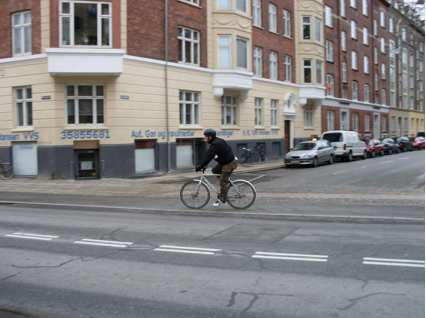
\includegraphics[scale=0.5]{billederogfigur/cykelsti.png}
  \end{adjustbox}
   \caption{Cykelsti}
 \end{figure}


En cykelbane er en bane, som deler vejen med kørebanen. Den er kun afgrænset mod kørebanen med 30 cm bred udbrudt kantlinje. Heraf har cykelbanen status som en cykelsti, og er ofte markeret med et rundt påbudsskilt eller med et cykelsymbol på vejen. En cykelbane etableres, hvis der kun er få cyklister, langsomt kørende biler, ved økonomiske eller pladsmæssige årsager \footnote{http://www.koreskoleservice.dk/Resources/Files/download/vejafm%C3%A6rkning/anvendelse/BEKnr801af04-07-2012.pdf 03/12-2015}. 
  Ifølge bekendtgørelsen om anvendelse af afmærkninger, kan almindelige vognbaner adskille sig fra blandt andet cykelbaner, hvor kantlinjen skal udføres bred \footnote{http://pvr.as/cykelstier-i-kobenhavn/ 03/12-2015}.  Det koster 500.0000 kroner at afmærke en kilometer cykelbane.  

\subsection{Cykelbane i Nytorv/Østerågade}
En cykelbane i Nytorv/Østerågade kan en cykelbane ifølge interviewpersonerne bl.a. udløse mere tryghed i området (se bilag), da der på nuværende tidspunkt er manglende vejplads til cyklisterne. Herved kunne den generelle cykelsti udformes som følgende ruteplan. Målene og billedet er taget fra http://iform.dk/ruteplanner/tegn.

RUTEPLAN BILLEDE
\begin{figure}[htbp]
   \label{fig:Ruteplan}
   \centering
   \begin{adjustbox}{max width=\textwidth}
     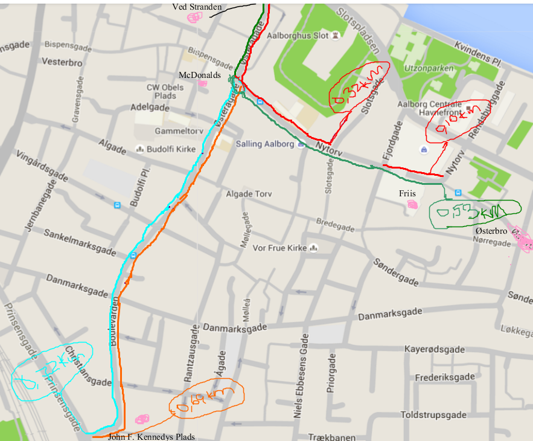
\includegraphics[scale=0.5]{billederogfigur/ruteplanlaegning.png}
  \end{adjustbox}
   \caption{Ruteplanlægning}
 \end{figure}
Cykelbanen kunne laves fra enden af Friis til Ved Stranden på højre og venstre side, rundt om pladsen foran McDonalds, også videre mod Boulevarden til John F. Kennedys Plads, da der også er mindre vejplads til cyklisterne i det område. Følgende billeder er taget fra https://www.google.com/maps. 

3 BILLEDER MANGLER
\begin{figure}[htbp]
   \label{fig:Cykelsti}
   \centering
   \begin{adjustbox}{max width=\textwidth}
     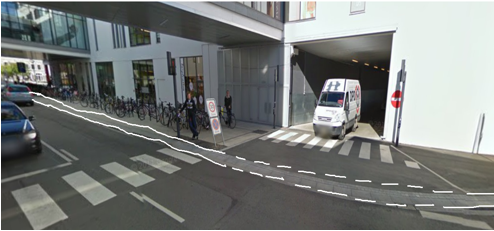
\includegraphics[scale=0.2]{billederogfigur/ved_friis.png}
  \end{adjustbox}
   \caption{Cykelsti ved Friis}
 \end{figure}

\begin{figure}[htbp]
   \label{fig:Cykelsti_ved_Friis}
   \centering
   \begin{adjustbox}{max width=\textwidth}
     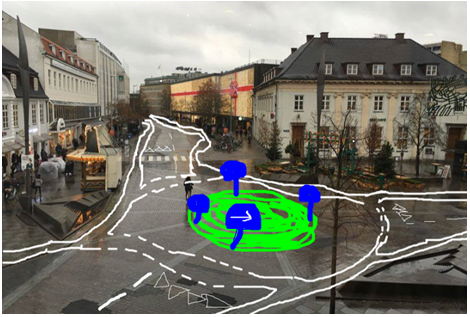
\includegraphics[scale=0.2]{billederogfigur/cykelsti_ved_mac.png}
  \end{adjustbox}
   \caption{Cykelsti ved Friis}
 \end{figure}

\begin{figure}[htbp]
   \label{fig:Cykelsti_mod_Boulevarden}
   \centering
   \begin{adjustbox}{max width=\textwidth}
     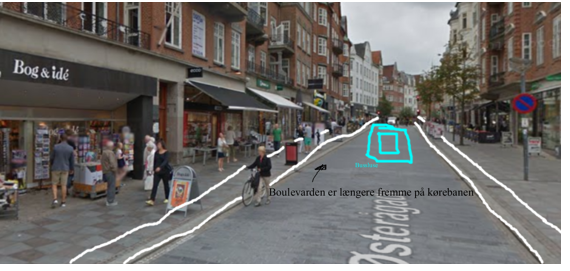
\includegraphics[scale=0.2]{billederogfigur/bogogide.png}
  \end{adjustbox}
   \caption{Cykelsi mod Boulevarden}
 \end{figure}


Ved Østerbro er der blevet lavet en cykelbane midt på fortovet, på samme måde kunne en cykelbane i de ovenstående områder laves. Billedet er taget af Fatimahs mobil.

CYKELSTI VED ØSTERBRO
\begin{figure}[htbp]
   \label{fig:Cykelsti ved Østerbro}
   \centering
   \begin{adjustbox}{max width=\textwidth}
     \includegraphics[scale=0.2]{billederogfigur/østerbro.png}
  \end{adjustbox}
   \caption{Cykelsti ved Østerbro}
 \end{figure}

\subsection{Vurdering af løsning på problemet i Nytorv/Østerågade}
Fordelen ved at etablere en cykelsti eller cykelbane er, at hver trafikantgruppe vil føle sig mere trygge af at de var delt. Ifølge en interviewperson bliver folk utrygge af, at”(…) fodgængere, cyklister og biler nærmest deler vejen, og at det ikke alle der tager hensyn til hinanden, vil føle mig mere tryg hvis vi var delt. ” En differentiering mellem trafikantgrupperne vil virke mere betryggende, end hvis de forskellige trafikantgrupper skulle dele vejen, her af vil det være en fordel at få etableret en cykelbane med kantlinjer frem for en cykelsti med en kantsten eller en rabat, da det er markant billigere, at få udført en cykelbane. Ulempen ved at have en cykelbane er at der cykler mange ud imod området, det mener en interviewperson, at “(…)om morgenen så er der fart på her i området, altså mange folk cykler mod skoler, universitet og på arbejde(…)”. Det vil i vissetilfælde resultere i, at cykelbanen bliver proppet og at cyklisterne vil fordele sig på kørebanen og længere ud på fortovet. I den forstand vil cykelbanen ikke afvikle morgentrafikken godt nok. Heraf kunne en cykelbro være mere praktisk men dog vil den være dyr at finansiere.   
\\

BILLEDER, KILDEHENVISNING OG GENERELLE RETTELSER MANGLER


